\chapter{Исследовательская часть}

В данном разделе будут приведены примеры работы программы, а также проведен сравнительный анализ алгоритмов при различных ситуациях на основе полученных данных.

\section{Технические характеристики}

Технические характеристики устройства, на котором выполнялось тестирование представлены далее:
\begin{itemize}[label={---}]
	\item операционная система: Windows 11, x64;
	\item оперативная память: 8 Гб;
	\item процессор: AMD Ryzen 5 5500U с видеокартой Radeon Graphics 2.10~ГГц.
\end{itemize}

Во время замеров времени ноутбук был нагружен только встроенными приложениями окружения.

\section{Демонстрация работы программы}

На рисунке~\ref{img:run} представлен результат работы программы.

\begin{figure}[H]
	\center{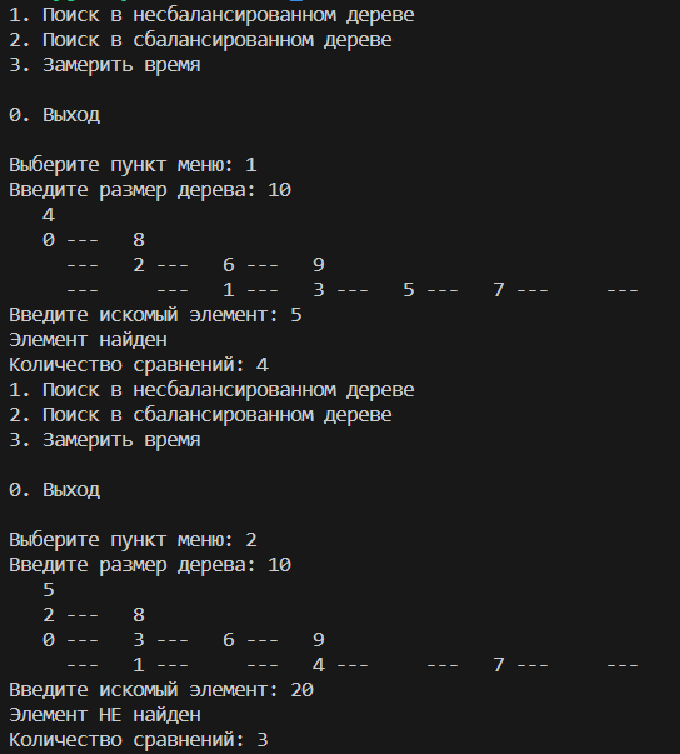
\includegraphics[scale=1.5]{img/run}}
	\caption{Пример работы программы}
	\label{img:run}
\end{figure}
\clearpage

\section{Количество сравнений при поиске элемента}

Результаты замеров приведены в таблице~\ref{tbl:time_mes}.

\begin{table}[H]
	\begin{center}
		\begin{threeparttable}
			\captionsetup{justification=raggedright, singlelinecheck=off}
			\caption{Результаты замеров количества сравнений}
			\label{tbl:time_mes}
			\begin{tabular}{|r|r|r|}
				\hline
				\begin{tabular}{c}
					Количество\\элементов\\в дереве
				\end{tabular} & \begin{tabular}{c}
				Количество\\сравнений\\в АВЛ-дереве
				\end{tabular} & \begin{tabular}{c}
				Количество\\сравнений\\в двоичном дереве
				\end{tabular} \\ \hline
				128 & 8 & 14\\\hline
				256 & 9 & 17\\\hline
				512 & 10 & 18\\\hline
				1024 & 11 & 21\\\hline
				2048 & 12 & 27\\\hline
			\end{tabular}
		\end{threeparttable}
	\end{center}
\end{table}


На рисунке~\ref{img:graph} приведена визуализация результатов замеров.

\inputPdf{graph}{Визуализация результатов замеров}

\section{Вывод}

Как видно из графика \ref{img:graph}, при поиске в АВЛ-дереве выполняется меньше сравнений. Например, при количестве элементов в дереве 1024 и более количество сравнений в АВЛ-дереве в 2 раза меньше количества сравнений в двоичном дереве. Связано это с тем, что высота АВЛ-дерева меньше высоты двоичного дерева с тем же количеством элементов, а значит требуется меньшее количество сравнений.